\documentclass[conference]{IEEEtran}
\IEEEoverridecommandlockouts
\usepackage{cite}
\usepackage{amsmath,amssymb}
\usepackage{graphicx}
\usepackage{booktabs}
\usepackage{array}
\usepackage{longtable}
\usepackage{url}
\graphicspath{{figures/}}

\title{DeltaShot: Reference-Conditioned Neural Compression for UI Screenshot Sequences}
\author{\IEEEauthorblockN{Rithun K P, Balagopal V, and Saavan Rajeev}
\IEEEauthorblockA{B.Tech. Computer Science and Engineering (Artificial Intelligence)\\
Amrita Vishwa Vidyapeetham, Amritapuri, India\\
AM.SC.U4AIE24041, AM.SC.U4AIE24012, AM.SC.U4AIE24065}}

\begin{document}
\maketitle

\begin{abstract}
Platforms used for visual regression testing and versioned documentation often store a previous screenshot before a new version arrives. This report studies whether a learned image codec can use that earlier screenshot as side information when encoding a new screenshot, while retaining a standalone no-reference fallback. DeltaShot compares a CompressAI ScaleHyperprior No-Reference control with a v1 Reference-Conditioned wrapper using feature concatenation and a per-image Mode Selection rule. Experiments use a balanced, WebSight-derived mutation dataset of 24,000 rendered 512$\times$512 screenshot pairs. Both learned codecs were trained for 28 epochs on 20,000 training pairs per epoch with 128$\times$128 crops, batch size four, Adam at $10^{-4}$, and one rate-distortion weight $\lambda=0.0130$. The stored learned-codec evaluation contains 500 held-out pairs (100 in each of five change buckets); neural bpp is estimated from model likelihoods. Reference conditioning has lower estimated bpp than the No-Reference control in all five buckets, with mean PSNR differences from $-0.07$ to $-0.54$ dB. The unrelated-bucket Mode Selection correctness check passes on all 100 evaluated pairs under the stored rate-distortion objective. These are preliminary, single-operating-point results on synthetic mutation data. The available artifacts do not establish a learned-codec RD curve, BD-rate, full-test learned-codec performance, or generalization to real product histories.
\end{abstract}

\begin{IEEEkeywords}
learned image compression, screenshot compression, side information, rate-distortion, UI screenshots
\end{IEEEkeywords}

\section{Introduction}
Screenshot sequences occur in visual regression testing, continuous integration artifacts, and versioned documentation. In these settings, the system often already stores an earlier screenshot of the same page. Independent codecs such as JPEG and WebP do not use that stored image as side information. DeltaShot explores conditional coding: encode a target screenshot while both encoder and decoder have access to a reference screenshot.

The core question is: at matched reconstruction quality, can a target become smaller when encoded using a useful reference than when encoded independently, and can the system avoid a worse rate-distortion choice when the reference is unrelated? The present implementation addresses this question with an independently trained No-Reference control, a Reference-Conditioned v1 codec, and a mode selector.

The contribution is narrower than general screen-content compression. Domain-specialized screen-content coding has already been studied, including learned models for screen-content images \cite{heris2023}. Reference-conditioned compression has also been studied for video and correlated stereo imagery \cite{li2021,mital2023}. DeltaShot focuses on sparse UI screenshot histories, where reference/target similarity can vary from identical to unrelated. The current implementation is v1 feature concatenation; it does not implement cross-attention.

\section{Dataset}
\subsection{Source and construction}
The source pages are WebSight v0.2 pages. The project renders each HTML page and creates a reference/target pair by applying one of six operators: color change, text change, layout change, insertion, removal, or replacement. The resulting examples are rendered screenshots, not captured histories of actual products. Reported performance is therefore scoped to this WebSight-derived mutation dataset.

Each pair is assigned a degree-of-change bucket using the changed-pixel ratio. The five balanced buckets are identical, minor, moderate, major, and unrelated. The unrelated bucket uses unrelated pages; the other buckets are generated by the mutation/rendering pipeline. Representative test pairs were spot-checked against their metadata according to the project runbook.

\begin{table}[t]
\caption{Dataset split and bucket counts}
\label{tab:dataset}
\centering
\footnotesize
\begin{tabular}{lrrrrrr}
\toprule
Split & Total & Ident. & Minor & Mod. & Major & Unrel.\\
\midrule
Train & 20,000 & 4,000 & 4,000 & 4,000 & 4,000 & 4,000\\
Validation & 2,000 & 400 & 400 & 400 & 400 & 400\\
Test & 2,000 & 400 & 400 & 400 & 400 & 400\\
\bottomrule
\end{tabular}
\end{table}

All images are RGB screenshots stored at 512$\times$512. Training samples are cropped to 128$\times$128. The learned evaluation uses a stratified subset of 100 test pairs per bucket (500 total). Classical and generic pretrained CompressAI baselines use the full 2,000-pair test set.

\section{System}
\subsection{No-Reference control}
The control codec is CompressAI's \texttt{ScaleHyperprior} with quality-3 channel configuration $N=128$, $M=192$ \cite{balle2018}. It receives only the target image. The analysis transform maps pixels to latent variables, the hyperprior models their distributions, and entropy coding stores quantized latents. The synthesis transform reconstructs an RGB image. The base transforms and GDN operations are supplied by CompressAI rather than handwritten in this repository.

\subsection{Reference-Conditioned v1}
The Reference-Conditioned model wraps the same ScaleHyperprior base. A shared reference feature extractor reuses early analysis-transform layers and yields feature maps at three scales. In v1, the deepest feature is resized to the target latent grid and projected with a 1$\times$1 convolution. The projected reference feature is concatenated with target features. Learned 1$\times$1 fusion layers condition the analysis, entropy-scale prediction, and synthesis paths.

The decoder requires the same reference image used by the encoder. No cross-attention, motion estimation, or geometric image warping is implemented in v1. This lightweight version is a first test of reference use, not a solution to arbitrary spatial alignment.

\subsection{Mode Selection}
The evaluation-time selector compares the stored likelihood-rate objective:
\begin{align}
J_{\mathrm{N}} &= \widehat{R}_{\mathrm{N}}+\lambda D_{\mathrm{N}},\\
J_{\mathrm{R}} &= \widehat{R}_{\mathrm{R}}+\frac{1}{HW}+\lambda D_{\mathrm{R}},
\end{align}
where $\widehat{R}$ is likelihood-estimated bpp, $D$ is RGB mean-squared error on normalized pixels, and $1/(HW)$ accounts for a one-bit reference-mode indicator. The lower-cost mode is selected. The live demo has a separate bitstream-level selector that uses actual file bytes; its results are not the 500-pair evaluation reported here.

\section{Training and Experimental Protocol}
Both learned models use the same seed (24041), training split, 20,000 training pairs per epoch, crop size 128, batch size four, Adam learning rate $10^{-4}$, 28 epochs, and $\lambda=0.0130$. Training was run on CPU with mixed precision disabled. The loss is CompressAI's MSE rate-distortion loss, combining estimated rate and lambda-weighted distortion. This is a single operating point.

The generic learned baseline is the pretrained CompressAI \texttt{bmshj2018-hyperprior} evaluated at qualities 1, 3, 5, and 7. Classical JPEG and WebP were run at qualities 10, 25, 50, 75, and 90; Delta+PNG was evaluated as a lossless reference-difference path. These baselines have 2,000 test records per configuration. For the 500-pair matched comparison, rows are joined by exact pair ID. Classical settings shown as quality-matched are the nearest finite mean-PSNR setting to the Reference-Conditioned mean within that bucket. The complete full-test quality sweep is included in Appendix A.

\subsection{Metrics}
Bits per pixel (bpp) is encoded bits divided by image pixels. For the learned 500-pair evaluation, bpp is estimated from model likelihoods, not measured from serialized bitstreams. PSNR is computed against the target in dB. MS-SSIM measures structural similarity. MSE is the squared pixel error used in the rate-distortion objective. Classical baseline artifacts do not contain MS-SSIM; those cells are unavailable, not zero. Delta+PNG is lossless, so lossy distortion metrics are not applicable.

A full BD-rate computation requires multiple RD operating points and a defined comparable quality range. Only one learned lambda is available; therefore, BD-rate and a complete learned RD curve are not reported.

\section{Results}
\subsection{Learned codec metrics}
Table~\ref{tab:learned} reports every bucket and all three learned modes. Each row represents 100 test pairs. Values are means over the stored evaluation records. Mode Selection's measured output corresponds to its chosen mode.

\begin{table*}[t]
\caption{Learned codec results on the stratified 500-pair subset. Neural rate is likelihood-estimated bpp.}
\label{tab:learned}
\centering
\scriptsize
\begin{tabular}{llrrrrr}
\toprule
Bucket & Method & $n$ & Estimated bpp & PSNR (dB) & MS-SSIM & MSE\\
\midrule
Identical & No-Reference & 100 & 0.382124 & 36.0670 & 0.998557 & 0.00026593\\
& Reference-Cond. & 100 & 0.277259 & 35.9946 & 0.998568 & 0.00027071\\
& Mode Selection & 100 & 0.277262 & 35.9946 & 0.998568 & 0.00027071\\
\midrule
Minor & No-Reference & 100 & 0.362088 & 35.8694 & 0.998284 & 0.00028362\\
& Reference-Cond. & 100 & 0.264684 & 35.7122 & 0.998232 & 0.00029314\\
& Mode Selection & 100 & 0.264688 & 35.7122 & 0.998232 & 0.00029314\\
\midrule
Moderate & No-Reference & 100 & 0.290533 & 37.6219 & 0.997781 & 0.00026737\\
& Reference-Cond. & 100 & 0.219878 & 37.0803 & 0.997903 & 0.00028025\\
& Mode Selection & 100 & 0.219812 & 37.3437 & 0.997902 & 0.00028020\\
\midrule
Major & No-Reference & 100 & 0.448523 & 34.2946 & 0.994774 & 0.00051214\\
& Reference-Cond. & 100 & 0.359890 & 33.8913 & 0.995493 & 0.00052490\\
& Mode Selection & 100 & 0.359373 & 33.9847 & 0.995325 & 0.00053704\\
\midrule
Unrelated & No-Reference & 100 & 0.398917 & 35.8687 & 0.998535 & 0.00027625\\
& Reference-Cond. & 100 & 0.308683 & 35.3971 & 0.998494 & 0.00030885\\
& Mode Selection & 100 & 0.308686 & 35.3971 & 0.998494 & 0.00030885\\
\bottomrule
\end{tabular}
\end{table*}

Reference conditioning has lower estimated bpp than No-Reference in each bucket, with PSNR lower by 0.072, 0.157, 0.542, 0.403, and 0.472 dB for identical through unrelated, respectively. This is a rate/distortion trade-off at one lambda, not evidence of superiority at matched quality.

\subsection{Classical quality matching on the same 500 pairs}
Table~\ref{tab:matched} reports the selected finite-PSNR baseline settings and their gaps from Reference-Conditioned mean PSNR. Every selected classical setting has lower mean PSNR than Reference-Conditioned; thus, the rate comparison is not a matched-quality win. JPEG has no finite mean-PSNR setting in moderate and major because some source records are exact reconstructions, making the arithmetic mean PSNR infinite for every JPEG quality in those buckets.

\begin{table*}[t]
\caption{Nearest finite-PSNR classical/generic settings on the same 500 pair IDs. Gaps are baseline PSNR minus Reference-Conditioned PSNR.}
\label{tab:matched}
\centering
\scriptsize
\begin{tabular}{llrrr}
\toprule
Bucket & Codec / setting & Bpp & PSNR (dB) & Gap (dB)\\
\midrule
Identical & JPEG q90 & 1.39886 & 29.25154 & -6.74307\\
& WebP q90 & 0.98357 & 29.54462 & -6.44998\\
& CompressAI q7 & 0.99147 & 29.91445 & -6.08015\\
& Delta+PNG (lossless) & 0.09128 & lossless & n/a\\
\midrule
Minor & JPEG q90 & 1.32618 & 29.50879 & -6.20345\\
& WebP q90 & 0.93008 & 29.83399 & -5.87825\\
& CompressAI q7 & 0.93782 & 30.38984 & -5.32240\\
& Delta+PNG (lossless) & 0.18520 & lossless & n/a\\
\midrule
Moderate & JPEG & unavailable & unavailable & unavailable\\
& WebP q25 & 0.29919 & 30.34841 & -6.73189\\
& CompressAI q7 & 0.74473 & 32.65950 & -4.42080\\
& Delta+PNG (lossless) & 1.14652 & lossless & n/a\\
\midrule
Major & JPEG & unavailable & unavailable & unavailable\\
& WebP q25 & 0.45397 & 27.56176 & -6.32951\\
& CompressAI q7 & 1.11975 & 29.72162 & -4.16966\\
& Delta+PNG (lossless) & 2.76222 & lossless & n/a\\
\midrule
Unrelated & JPEG q90 & 1.46157 & 28.90886 & -6.48823\\
& WebP q90 & 1.03129 & 29.19466 & -6.20243\\
& CompressAI q7 & 1.03413 & 29.59043 & -5.80666\\
& Delta+PNG (lossless) & 2.62737 & lossless & n/a\\
\bottomrule
\end{tabular}
\end{table*}

\subsection{Full-test classical and generic learned baselines}
The full-test baseline runs include 2,000 pairs (400 per bucket) for every codec configuration. Table~\ref{tab:fulloverall} shows overall means. The generic CompressAI q1--q7 sweep trades increased bitrate for improved PSNR in the aggregate. Some JPEG/WebP settings have infinite mean PSNR because exact reconstructions are present in the source rows; the count is reported. Appendix A gives every per-bucket setting.

\begin{table}[t]
\caption{Full 2,000-pair test-set baseline means}
\label{tab:fulloverall}
\centering
\scriptsize
\begin{tabular}{llrrr}
\toprule
Codec & Setting & Mean bpp & Mean PSNR (dB) & $+\infty$ rows\\
\midrule
JPEG & q10 & 0.29211 & $+\infty$ & 16\\
JPEG & q25 & 0.47180 & $+\infty$ & 16\\
JPEG & q50 & 0.67088 & $+\infty$ & 16\\
JPEG & q75 & 0.92499 & $+\infty$ & 16\\
JPEG & q90 & 1.35979 & $+\infty$ & 16\\
WebP & q10 & 0.30993 & $+\infty$ & 16\\
WebP & q25 & 0.39678 & 28.28541 & 0\\
WebP & q50 & 0.53502 & $+\infty$ & 16\\
WebP & q75 & 0.64173 & $+\infty$ & 16\\
WebP & q90 & 0.95009 & $+\infty$ & 16\\
Delta+PNG & lossless & 1.35410 & lossless & 0\\
CompressAI & q1 & 0.17492 & 24.44661 & 0\\
CompressAI & q3 & 0.34325 & 26.96353 & 0\\
CompressAI & q5 & 0.54447 & 28.55544 & 0\\
CompressAI & q7 & 0.96421 & 30.44241 & 0\\
\bottomrule
\end{tabular}
\end{table}

\subsection{Mode Selection correctness check}
On the 100 unrelated evaluation pairs, Mode Selection was worse than the No-Reference objective on 0 pairs. Mean Mode Selection objective was $J=0.3086904281$, compared with $J=0.3989202306$ for No-Reference. The stored check therefore passes its stated criterion. This is a finite-subset correctness check under a likelihood-estimated objective; it is not a BD-rate guarantee and is not the live demo's actual-byte selector.

\begin{figure}[t]
\centering
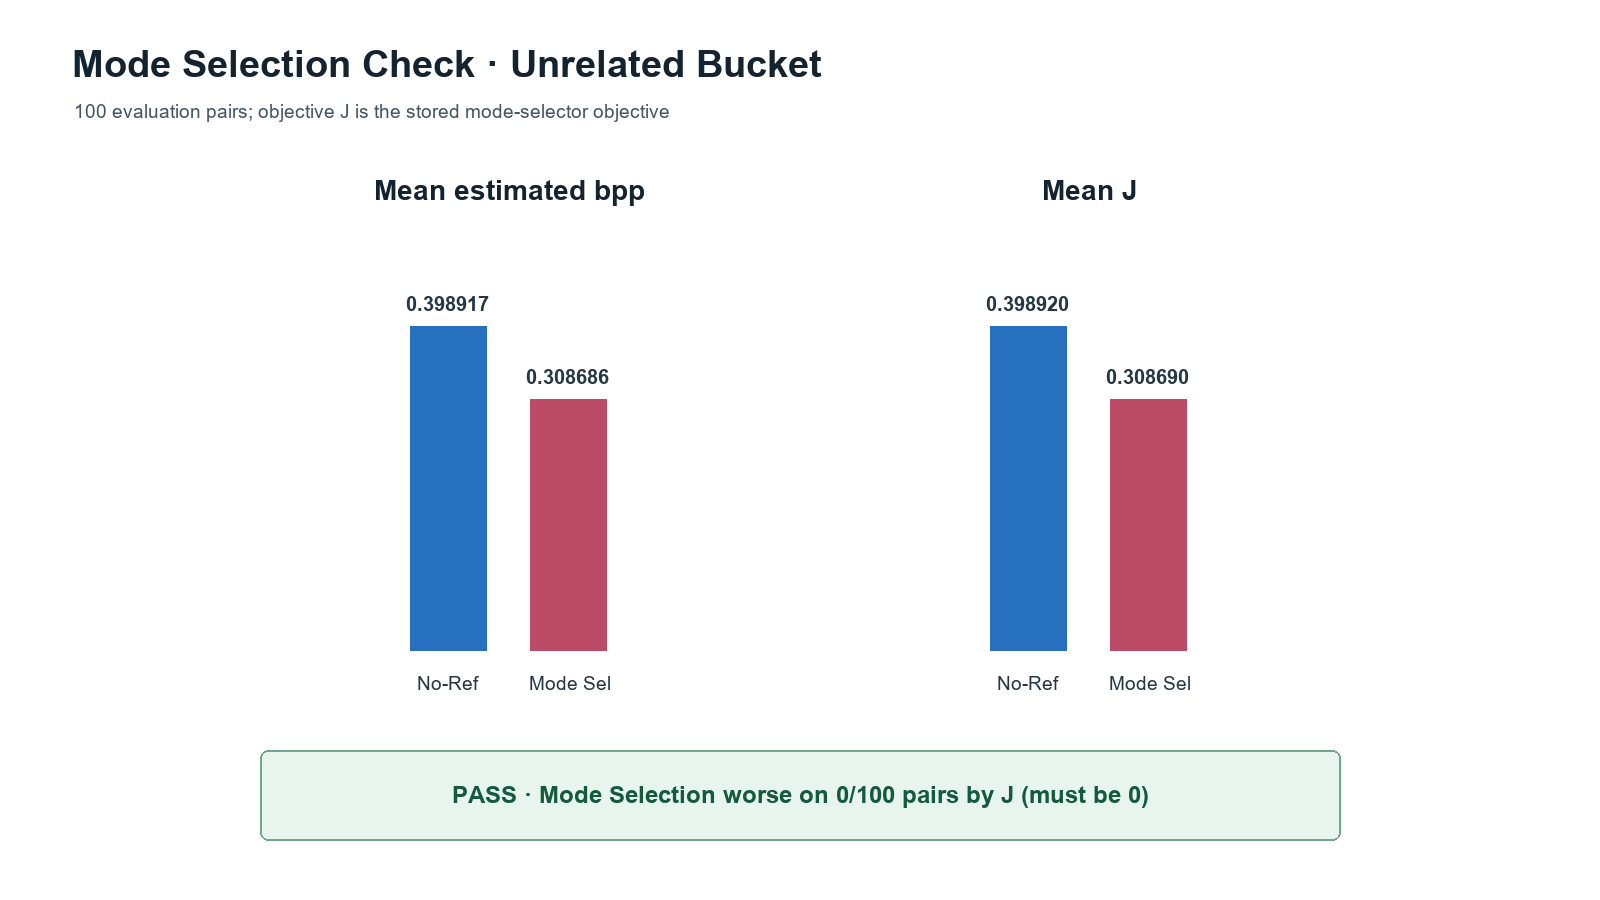
\includegraphics[width=\linewidth]{mode_selection_check.png}
\caption{Stored unrelated-bucket Mode Selection comparison.}
\label{fig:mode}
\end{figure}

\subsection{Training evidence}
Both training metric files contain 14,028 logged samples across zero-based epochs 0--27. Validation loss was not recorded. Figure~\ref{fig:loss} visualizes logged training loss; it must not be interpreted as validation performance or convergence proof.

\begin{figure}[t]
\centering
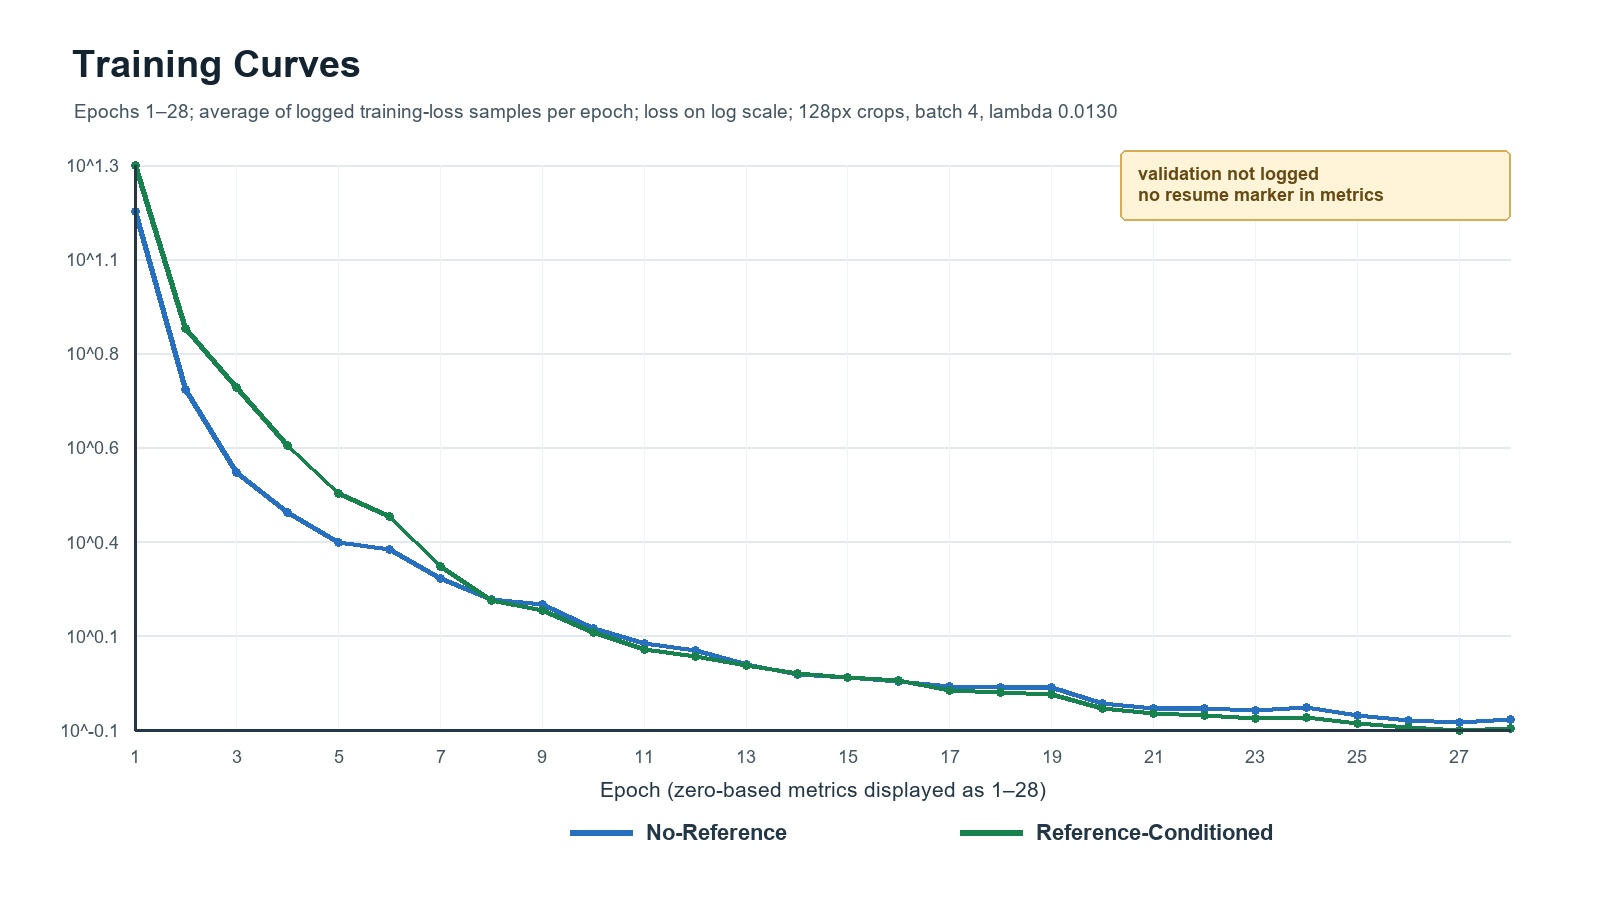
\includegraphics[width=\linewidth]{loss_curves.png}
\caption{Training loss history for the two learned codecs. Runs used 128-pixel crops, batch size four, and $\lambda=0.0130$.}
\label{fig:loss}
\end{figure}

\begin{figure*}[t]
\centering
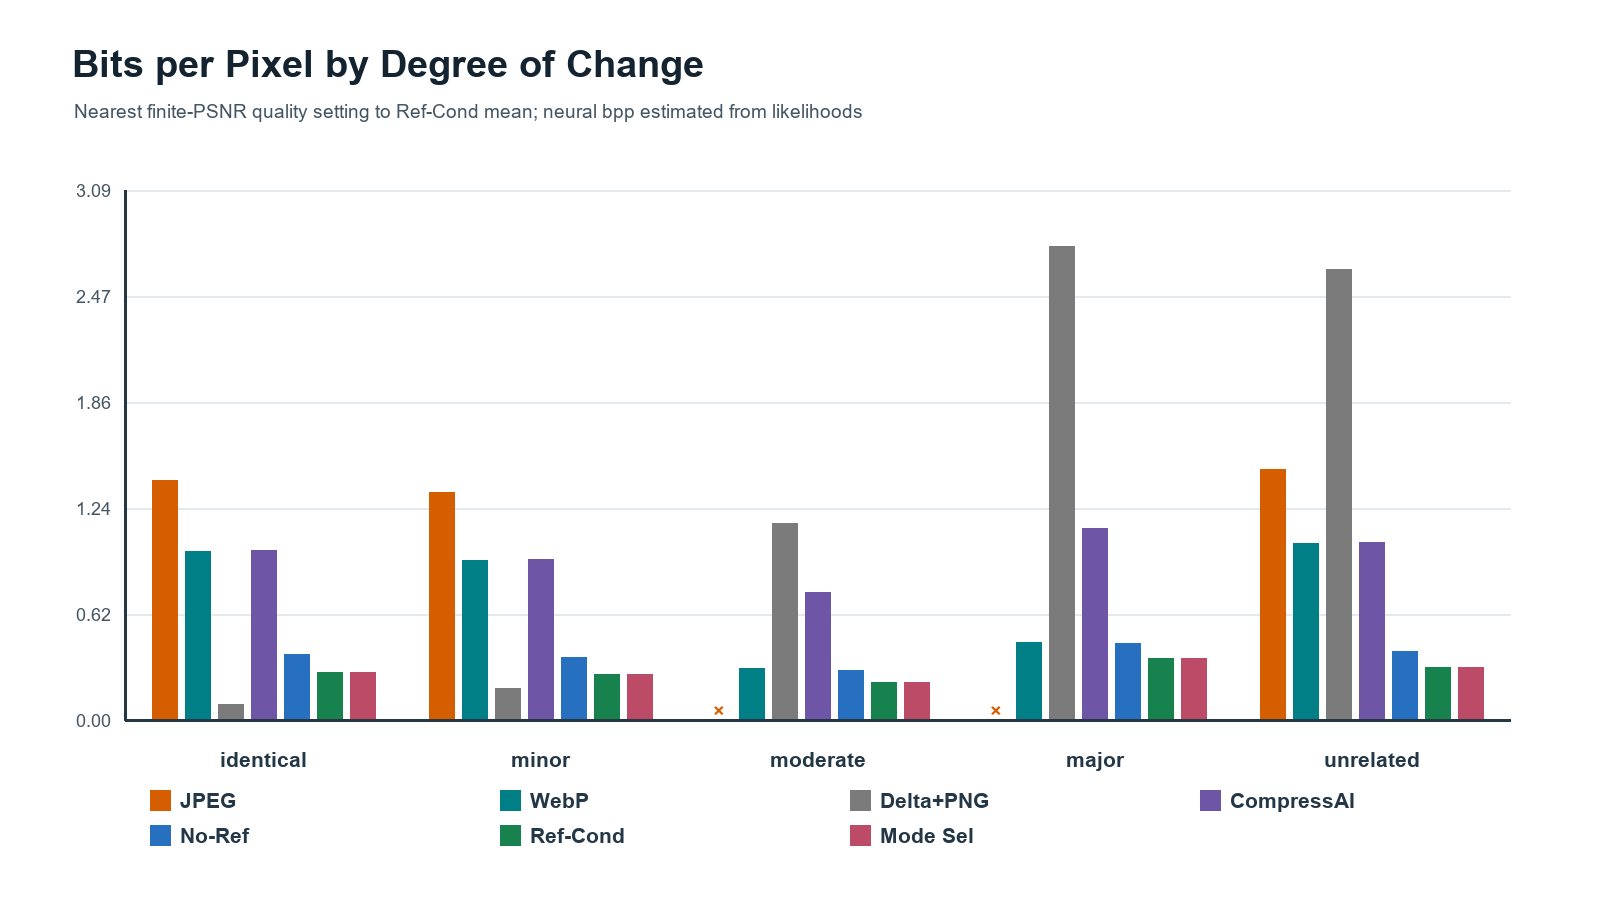
\includegraphics[width=0.86\textwidth]{bpp_by_bucket.png}
\caption{Rate comparison by change bucket on the 500-pair learned evaluation subset. Neural rates are likelihood estimates. Classical settings shown are selected by nearest finite mean PSNR to Reference-Conditioned within each bucket.}
\label{fig:bpp}
\end{figure*}

\section{Discussion}
The stored 500-pair evaluation supports a limited result: at $\lambda=0.0130$, Reference-Conditioned v1 has lower likelihood-estimated bpp than the matched No-Reference control in all five buckets, while its mean PSNR is modestly lower. Mode Selection satisfies the unrelated-bucket criterion for all 100 sampled unrelated pairs. These findings motivate further evaluation but do not show that the reference codec wins at matched quality.

The main limitations are:
\begin{itemize}
\item \textbf{Synthetic data:} all learned evaluation pairs are WebSight-derived generated mutations, not real site-version histories.
\item \textbf{Reduced learned evaluation:} learned codecs and Mode Selection were evaluated on 500 test pairs, not the full 2,000-pair test split.
\item \textbf{One lambda:} only one learned operating point is available. No learned RD curve or BD-rate can be computed.
\item \textbf{Estimated neural rate:} evaluation bpp is derived from likelihoods. The separate upload demo writes actual bitstreams, but its per-upload results are not the benchmark table here.
\item \textbf{Baseline metric gaps:} classical and generic CompressAI outputs do not contain MS-SSIM. Delta+PNG is lossless and is not meaningfully compared by lossy distortion metrics.
\item \textbf{Alignment:} Reference v1 uses simple resized feature concatenation, not cross-attention. The reference may not be spatially aligned with the target.
\item \textbf{No validation curve:} training logs contain sampled training losses but no validation-loss history.
\end{itemize}

Future work should add multiple matched lambda operating points, evaluate learned codecs over all 2,000 test pairs, publish per-bucket RD curves and BD-rate only after those curves exist, and validate on consented/licensed real screenshot histories split by site or product to avoid leakage.

\section{Conclusion}
DeltaShot implements a reference-conditioned screenshot codec prototype and a No-Reference control, together with a Mode Selection rule. Current artifacts show a lower likelihood-estimated rate for the conditioned model across five buckets at one operating point, with a small mean-PSNR trade-off, and a passing unrelated-bucket selection check on 100 sampled pairs. This is preliminary evidence limited to synthetic WebSight-derived mutations. It does not establish matched-quality superiority over JPEG/WebP, a full learned RD curve, BD-rate, or real-history generalization.

\clearpage
\onecolumn
\appendix
\section{Full-Test Baseline Quality Sweep by Bucket}
The following appendix contains all stored full-test aggregate baseline rows: JPEG and WebP qualities 10, 25, 50, 75, and 90; generic pretrained CompressAI qualities 1, 3, 5, and 7; and lossless Delta+PNG. Every row has 400 pairs within its bucket. Positive infinity counts indicate exact reconstructions, whose PSNR is infinite. Missing values are preserved as unavailable.
\begin{longtable}{llrrrr}
\caption{Full-test baseline sweep by bucket ($n=400$ per bucket).}\label{tab:fullsweep}\\
\toprule
Bucket & Codec & Setting & Mean bpp & Mean PSNR (dB) & $+\infty$ count\\
\midrule
\endfirsthead
\caption[]{Full-test baseline sweep by bucket (continued).}\\
\toprule
Bucket & Codec & Setting & Mean bpp & Mean PSNR (dB) & $+\infty$ count\\
\midrule
\endhead
\midrule
\multicolumn{6}{r}{Continued on next page}\\
\endfoot
\bottomrule
\endlastfoot
Identical & JPEG & q10 & 0.30088 & 23.99847 & 0\\
Identical & JPEG & q25 & 0.48642 & 25.87971 & 0\\
Identical & JPEG & q50 & 0.69213 & 27.26826 & 0\\
Identical & JPEG & q75 & 0.95472 & 28.38444 & 0\\
Identical & JPEG & q90 & 1.40398 & 29.24033 & 0\\
Identical & WebP & q10 & 0.32288 & 26.93090 & 0\\
Identical & WebP & q25 & 0.41323 & 27.89180 & 0\\
Identical & WebP & q50 & 0.55688 & 28.76584 & 0\\
Identical & WebP & q75 & 0.66752 & 29.14803 & 0\\
Identical & WebP & q90 & 0.98768 & 29.54137 & 0\\
Identical & Delta+PNG & lossless & 0.09127 & lossless & 0\\
Identical & CompressAI & q1 & 0.17998 & 24.09647 & 0\\
Identical & CompressAI & q3 & 0.35408 & 26.59840 & 0\\
Identical & CompressAI & q5 & 0.56090 & 28.05574 & 0\\
Identical & CompressAI & q7 & 0.99387 & 29.96323 & 0\\
Minor & JPEG & q10 & 0.28981 & 24.25878 & 0\\
Minor & JPEG & q25 & 0.46671 & 26.12276 & 0\\
Minor & JPEG & q50 & 0.66300 & 27.50276 & 0\\
Minor & JPEG & q75 & 0.91355 & 28.61358 & 0\\
Minor & JPEG & q90 & 1.34202 & 29.46360 & 0\\
Minor & WebP & q10 & 0.30825 & 27.16983 & 0\\
Minor & WebP & q25 & 0.39393 & 28.13527 & 0\\
Minor & WebP & q50 & 0.53064 & 29.00215 & 0\\
Minor & WebP & q75 & 0.63579 & 29.38478 & 0\\
Minor & WebP & q90 & 0.94099 & 29.77776 & 0\\
Minor & Delta+PNG & lossless & 0.18034 & lossless & 0\\
Minor & CompressAI & q1 & 0.17305 & 24.34036 & 0\\
Minor & CompressAI & q3 & 0.33913 & 26.85173 & 0\\
Minor & CompressAI & q5 & 0.53704 & 28.35808 & 0\\
Minor & CompressAI & q7 & 0.94965 & 30.28024 & 0\\
Moderate & JPEG & q10 & 0.24248 & $+\infty$ & 11\\
Moderate & JPEG & q25 & 0.38328 & $+\infty$ & 11\\
Moderate & JPEG & q50 & 0.53888 & $+\infty$ & 11\\
Moderate & JPEG & q75 & 0.73744 & $+\infty$ & 11\\
Moderate & JPEG & q90 & 1.07760 & $+\infty$ & 11\\
Moderate & WebP & q10 & 0.24360 & $+\infty$ & 11\\
Moderate & WebP & q25 & 0.30974 & 29.92951 & 0\\
Moderate & WebP & q50 & 0.41777 & $+\infty$ & 11\\
Moderate & WebP & q75 & 0.50047 & $+\infty$ & 11\\
Moderate & WebP & q90 & 0.74151 & $+\infty$ & 11\\
Moderate & Delta+PNG & lossless & 1.19121 & lossless & 0\\
Moderate & CompressAI & q1 & 0.14572 & 25.84081 & 0\\
Moderate & CompressAI & q3 & 0.27859 & 28.40452 & 0\\
Moderate & CompressAI & q5 & 0.43912 & 30.41447 & 0\\
Moderate & CompressAI & q7 & 0.76923 & 32.24756 & 0\\
Major & JPEG & q10 & 0.33043 & $+\infty$ & 5\\
Major & JPEG & q25 & 0.54347 & $+\infty$ & 5\\
Major & JPEG & q50 & 0.77919 & $+\infty$ & 5\\
Major & JPEG & q75 & 1.08026 & $+\infty$ & 5\\
Major & JPEG & q90 & 1.59519 & $+\infty$ & 5\\
Major & WebP & q10 & 0.35771 & $+\infty$ & 5\\
Major & WebP & q25 & 0.46144 & 27.52898 & 0\\
Major & WebP & q50 & 0.62345 & $+\infty$ & 5\\
Major & WebP & q75 & 0.75034 & $+\infty$ & 5\\
Major & WebP & q90 & 1.11083 & $+\infty$ & 5\\
Major & Delta+PNG & lossless & 2.79588 & lossless & 0\\
Major & CompressAI & q1 & 0.19889 & 23.79361 & 0\\
Major & CompressAI & q3 & 0.39687 & 26.29426 & 0\\
Major & CompressAI & q5 & 0.63448 & 27.83304 & 0\\
Major & CompressAI & q7 & 1.13367 & 29.70105 & 0\\
Unrelated & JPEG & q10 & 0.29694 & 24.05781 & 0\\
Unrelated & JPEG & q25 & 0.47913 & 25.94353 & 0\\
Unrelated & JPEG & q50 & 0.68121 & 27.32408 & 0\\
Unrelated & JPEG & q75 & 0.93900 & 28.43336 & 0\\
Unrelated & JPEG & q90 & 1.38015 & 29.28421 & 0\\
Unrelated & WebP & q10 & 0.31718 & 26.98605 & 0\\
Unrelated & WebP & q25 & 0.40557 & 27.94149 & 0\\
Unrelated & WebP & q50 & 0.54634 & 28.81133 & 0\\
Unrelated & WebP & q75 & 0.65451 & 29.19212 & 0\\
Unrelated & WebP & q90 & 0.96942 & 29.58484 & 0\\
Unrelated & Delta+PNG & lossless & 2.51183 & lossless & 0\\
Unrelated & CompressAI & q1 & 0.17693 & 24.16182 & 0\\
Unrelated & CompressAI & q3 & 0.34761 & 26.66875 & 0\\
Unrelated & CompressAI & q5 & 0.55081 & 28.11588 & 0\\
Unrelated & CompressAI & q7 & 0.97461 & 30.02000 & 0\\
\end{longtable}


\begin{thebibliography}{99}
\bibitem{balle2017}
J. Ball\'e, V. Laparra, and E. P. Simoncelli, ``End-to-end optimized image compression,'' in \emph{Proc. International Conference on Learning Representations (ICLR)}, 2017.
\bibitem{balle2018}
J. Ball\'e, D. Minnen, S. Singh, S. J. Hwang, and N. Johnston, ``Variational image compression with a scale hyperprior,'' in \emph{Proc. International Conference on Learning Representations (ICLR)}, 2018.
\bibitem{heris2023}
R. Zamanshoar Heris and I. V. Baji\'c, ``Multi-task learning for screen content image coding,'' in \emph{Proc. IEEE International Symposium on Circuits and Systems (ISCAS)}, 2023.
\bibitem{li2021}
J. Li, B. Li, and Y. Lu, ``Deep contextual video compression,'' in \emph{Advances in Neural Information Processing Systems}, vol. 34, pp. 18114--18125, 2021.
\bibitem{mital2023}
N. Mital, E. \"Ozy\i lkan, A. Garjani, and D. G\"und\"uz, ``Neural distributed image compression with cross-attention feature alignment,'' in \emph{Proc. IEEE/CVF Winter Conference on Applications of Computer Vision (WACV)}, 2023.
\end{thebibliography}
\end{document}
